% Author: Mathias Hablützel
% Interpretation und Validierung der Resultate

\section{Erweiterbarkeit}
% Zeigen, dass es leicht erweiterbar und wiederverwendbar ist.
\subsection{Wiederverwendbarkeit}
Java ist eine strikt objektorientierte Sprache und zwingt den Entwickler
Klassen zu entwickeln. Allerdings bedeutet das nicht, dass dadurch automatisch
auch modularer und wiederverwendbarer Code entsteht. Durch das geschickte
verwenden von Entwicklungsmustern kann man schon früh in der Planungsphase
sicherstellen, dass möglichst wiederverwendbarer Code entsteht. Ein gutes
Anschauungsbeispiel ist hier die Klasse \texttt{Bilinear.java}, dass eine
Implementation des Interfaces \texttt{InterpolationAlgorithm.java} ist. Das
Interface gibt einzig vor, welche Schnittstellen beziehungsweise welche
Methoden zu implementieren sind und in unserem Fall auch andere gewisse
Randbedingungen. Somit kann die Klasse für Interpolation einfach ausgetauscht
werden mit einem anderen Algorithmus, ohne das der Rest der Software betroffen
ist. Somit wäre es möglich komplexere Interpolationsverfahren zu nutzen, die
zum Beispiel spezialisierte Hardware wie ein FPGA\footnote{Field-programmable
gate array}, um eine noch schnellere Berechnung grosse Datensätze zu
ermöglichen.

\subsection{Parallelisierung}
% Aufzeigen, dass Paralellisierung möglich ist.
\subsubsection{Multi-Core-CPU}
Im Rahmen der Arbeit hat sich schnell die Frage gestellt, wie man die
Multi-Core-Architektur eines Supercomputer ausreizen kann. Die jetztige
Implementation verwendet eine reine Single-Thread-Archtitektur mit synchronen
Aufrufen. Das bedeutet einerseits, dass die nominelle Taktgrösse der CPU die
Verarbeitungsgeschwindigkeit direkt bestimmt und andererseits liegen die
anderen Cores brach und werden nicht benutzt. Da aber heute immer mehr CPUs
mit tieferen Taktraten dafür mehr Cores gebaut werden, vergeuden wir
eigentlich viel Leistungspotential.

Allerdings muss auch beachtet werden, dass solange die TDP\footnote{Thermal
Design Power, maximale Verlustleistung} nicht verbraucht wird, sich die
ungenutzten Cores abschalten und damit dem aktiven Core erlauben zu übertakten
und die verfügbare Verlustleistung auszureizen.  Jedoch muss erwähnt werden,
dass die Verlustleistung nicht linear mit der Rechenleistung zunimmt und es
damit kein sinnvoller Trade-Off darstellt, insbesondere wenn dadurch höchsten
30\% mehr Berechnung drin liegen gegenüber 400\% bei voller
Quad-Core-Berechnungen.

\subsubsection{Asynchronous Threads}
Auf der anderen Seite blockieren wir mit synchronen Methodenaufrufe die
Reaktionsfähigkeit der Benutzerinterfaces. Das heisst, dass der Benutzer ein
eingefrorenes Programm sieht, solange die Algorithmen beschäftig sind. Solche
Oberflächen gehören zu den Tabu-Design-Prinzipien: Ein Programm sollte dem
Anwender immer über seinen internen Zustand informieren und wissen lassen wie
weit seine Berechnungen schon getätigt wurden. Ein Benutzer könnte eine nicht
reaktive Oberfläche so missinterpretieren, dass die Software abgestürtzt ist,
sein Beenden erzwingt und die Berechnung unsinnigerweise von neuem anstösst.

Somit wäre es sinnvoll Threads mit Callback-Hooks zu erstellen, die in
regelmässigen Berechnungsabständen ihren Status melden. Wichtig ist hier, dass
die Häufigkeit von Rückmeldungen nicht von Timern also zeitabhängig ist. Viel
sinnvoller ist es, nach einer Anzahl von Operationen den Stand der
Berechnungen zu melden. Eine übliche Vorgehensweise ist die Anzahl
Berechnungen zu ermitteln und bei jedem Abschluss der Berechnung diese als
erfolgt zu markieren.

\subsubsection{MapReduce}
MapReduce\footnote{MapReduce ist eine Entwicklung von Google und ist als
Hadoop Mapreduce in einer OpenSource-Fassung verfügbar.} ist eine sehr
effiziente Möglichkeit für Clustercomputing die maximale
Berechnungsgeschwindigkeit zu verwenden. Das Problem wird solange in seine
Teilprobleme zerlegt, bis entweder jeder Knoten im Cluster beschäftigt ist
oder das Problem nicht mehr zerlegt werden kann. Danach werden die Resultate
wieder eingesammelt und der aufrufenden Komponente
bereitgestellt.\cite{Google:MapReduce}

\subsubsection{GPGPU\protect\footnote{\textbf{G}eneral-\textbf{p}urpose computing on \textbf{g}raphics \textbf{p}rocessing \textbf{u}nits}}
Eine weitere Stufe des Parallelisierung wäre das Verwenden von einer
Grafikkarte, die mit ihren vielen Shader-Kerne sehr viele Berechnungen
parallel ausführen kann. Insbesondere verfügen die Grafikkarten über solche
speziellen Interpolations-Stufen und können auch komplexere
Interpolationsalgorithmen in sehr kurzer Zeit ausführen.
 
\subsection{Weitere Datenquellen}
% Wie weitere Datenquellen eingesetzt werden können (z.B. HTTP anstatt Datei)
Zu einer späteren Zeit wäre es möglich die Informationen über Windfelder und
des Polardiagramms per HTTP oder andere Protokolle zu laden. Somit wäre es
möglich die aktuellen Windfelder von einem zentralen Server zu laden, der an
einem anderen physischen Standort ist, ohne per NFS darauf zuzugreifen.

\subsection{Website}
% Wie daraus eine Webseite gemacht werden kann. Apps?
Sobald die Applikation in die Infrastruktur der MeteoSchweiz integriert ist,
wäre die kommerzielle Verwendung mit einer Website oder über eine Mobile-App
eine interessante Bachelor-Arbeit. Der Benutzer würde dann zum Beispiel per
Mobile-App seine aktuelle Position mitteilen, sein Bootstyp auswählen und
seine Zielkoordinaten. Diese werden dann an den MeteoSchweiz-Server
übermittelt und die Berechnung angestossen. Die Resultate können dann entweder
als grafische Karte oder als Datei mit GPS-Koordinate ausgegeben werden. Da
die meisten Smartphones Google Maps installiert haben, können diese sehr
einfach das GPX-Dateiformat verwenden und die Route als Overlay darstellen.

\subsection{Isochronen}
In der Meteorologie bezeichnen Isochronen die Verbindungslinien der verschiedenen
Routen, die von einem Anfangspunkt aus in derselben Zeit zu erreichen sind. 
Für die Umsetzung dieser Erweiterung sollte eigentlich eine Dreisatz-Berechnung
genügen. Da wir zu jedem Knoten die Dauer der Fahrt haben, braucht man nur
noch festzustellen, zwischen welchen Spalten diese Zeit der Isochronen zu kommen
hat. Nachdem dies herausgefunden wurde, wird anhand der Länge der Strecke
zwischen diesen beiden Spalten ein Dreisatz gebildet, welches uns die Länge bis zum Isochron 
liefert. Zum Schluss brauchts nur noch den Punkt zu zeichnen.

Umgesetzt sollte es ungefähr so aussehen:

\begin{figure}[h!]
\centering
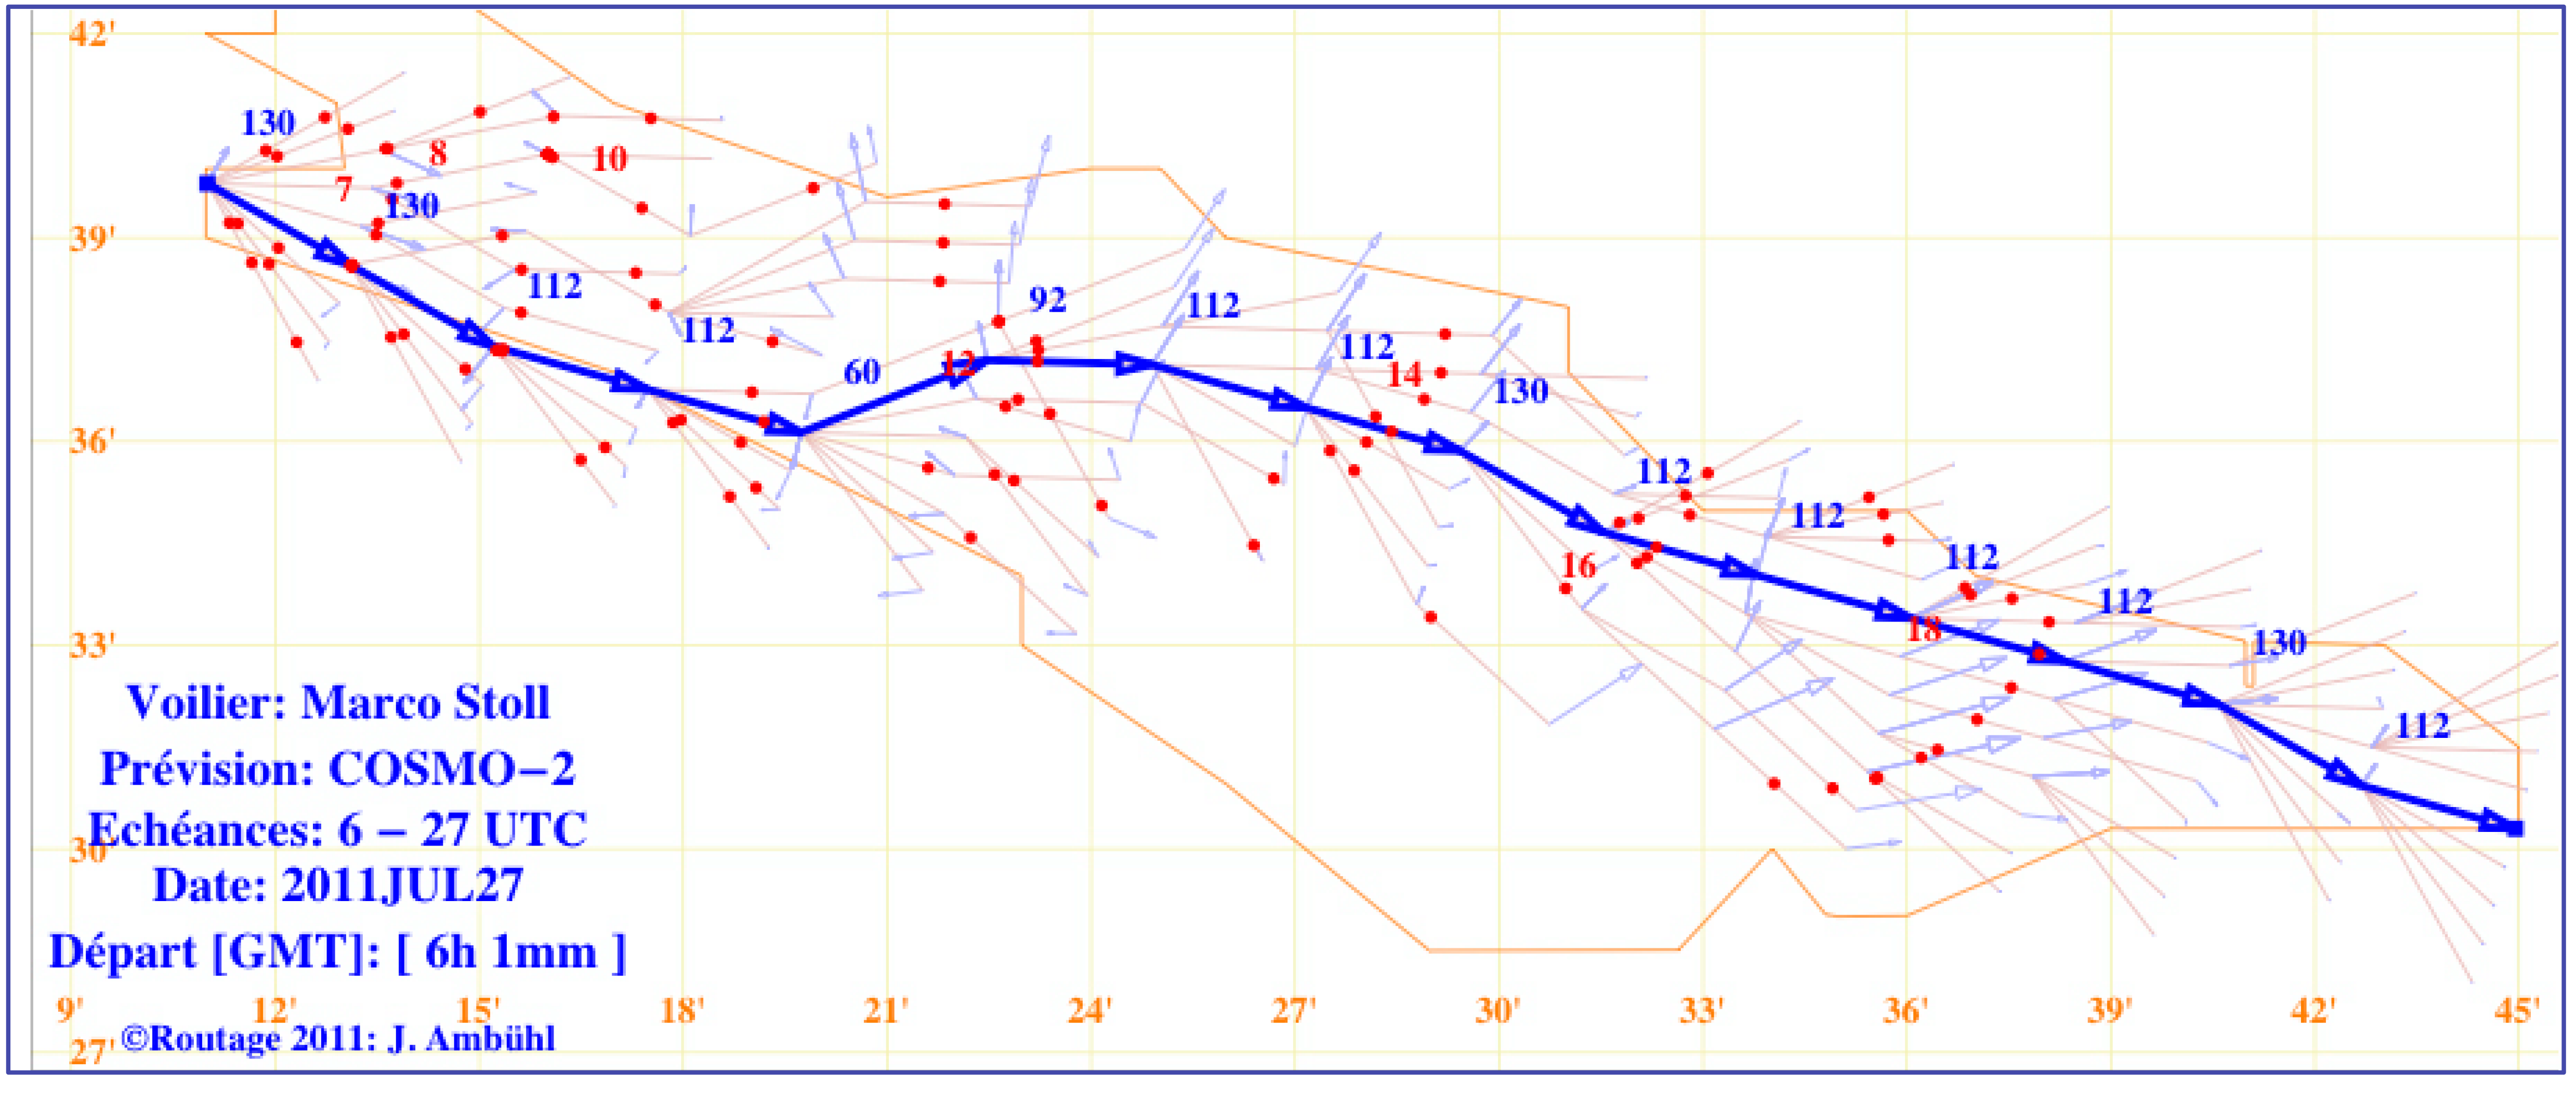
\includegraphics[width=1\linewidth]{img/isochronen}
\caption{Isochronen zu gegeben Zeiten}
\label{isochron}
\end{figure}

\section{Programmiertechnische Grenzen}
% (Im Sitzungsprotokoll vom 06.03.2012, Punkt 3)
%% 3. Im Bericht sollte ein Absatz vorhanden sein, welches die 
%% programmiertechnischen Grenzen oder Genauigkeiten der mathematischen 
%% Funktionen wie Sinus/Cosinus, Datentypen etc. behandelt und diskutiert. 
\subsection{Double-Genauigkeit}
Intern verwendet Double die \texttt{IEEE 754}-Arithmetik und beschränkt damit
die Genauigkeit der Zahlen und Berechnungen. Allerdings reicht die Genauigkeit
für unsere Zwecke zu genüge aus, da wir nie in einen Grenzbereich des
Double-Datentyps kommen. Die kleinste Zahl für die Windgeschwindigkeit ist ja
auf $0.0001$ limitiert worden. Unvernünftig grosse Werte erwarten wir sowieso
nicht, somit stellen diese Beschränkungen keine Probleme dar.

\subsection{Berechnungsgenauigkeit von primitiven Mathematikfunktionen}
Intern werden die die Resultate für die Sinus- und Cosinus-Funktionen in
Lookup-Tabellen abgespeichert und bei der Abfrage durchlaufen. Da wir nicht
eine Präzision von mehreren Nachkommastellen benötigen, reicht die vorhandene
Präzision. Dazu kommt, dass ein Segelboot unter keinen Umständen den Kurs auf
zwei Nachkommastellen halten kann.

\section{Sonderfälle}
\subsection{Unvollständiger Entscheidungsbaum bei zu kleinem Spread-Faktor}
Es ist ein Fall bekannt, bei denen die Berechnungen zwar korrekt terminieren,
aber der Entscheidungsbaum unvollständig wird. Für den Knoten \texttt{k} wird
nun der optimale Vorgänger berechnet und gespeichert sofern dieser innerhalb
des angegebenen Spread liegt.

Allerdings könnte ein Spezialfall eintreten, bei dem der letzte
Vorgängerknoten der optimale Vorgänger ist, allerdings ausserhalb des Spreads
liegt. Dann wird dieser nämlich als optimaler Vorgänger gespeichert mit
\texttt{MAX\_TOA} als Adjazenzgewicht. Allerdings scheitert wird die Abfrage
in Zeile \ref{sloc:verifyspread} des Listings \ref{lst:decisionspreadbug} und
der Vorgänger wird nicht in \texttt{GraphList} gespeichert, was zu einem
Knoten ohne Vorgänger führt und damit zu einem NullPointer.

\begin{lstlisting}[caption={Schwer zu findender Bug in
Decision.java},label=lst:decisionspreadbug,escapeinside={@}{@}]
for (int j = 0; j < getMaxj(); j++) {
        travelDistance[j] = calcTravelDistance(r, j, k, windfieldNo);
        
        /*
         * Saves the minimum distance and makes sure that the node is in
         * the spread.
         */
        if (travelDistance[j] < maxTimeOfArrival) {
        	/*
        	 * Checks, if the position of the shortest distance is legal
        	 * based on spread. If not, it sets the default distance.
        	 */
        	if (Math.abs(k - j) <= spread) {
        		maxTimeOfArrival = travelDistance[j];
        		position[k][__ROW__] = j;
        		position[k][__TRAVELTIME__] = travelDistance[j];
        	} else {
        		position[k][__ROW__] = j;
        		position[k][__TRAVELTIME__] = MAX_TOA;
        	}
        }
}

@\label{sloc:verifyspread}@ if (Math.abs(k - (int) position[k][__ROW__]) <= spread) {
       /*
        * SNIP
        */
       graphList.get(r).get(k).setTimeOfArrival(position[k][__TRAVELTIME__]);
       graphList.get(r).get(k).setPrevious(graphList.get(r - 1).get((int) position[k][__ROW__]));
}

\end{lstlisting}

\subsection{Falsche Hysterese-Berechnung}
Ein weiterer schwer zu findender Bug ist eine unvollständige
Hysterese-Berechnung in \texttt{Decision.java}. Wie Listing
\ref{lst:hysterisisbug} zeigt, wird berechnet um wie viele Windfelder der
Algorithmus in der Zeit nach vorne springen soll, wenn die Reisezeit mehr als
30 Minuten beträgt. Nehmen wir also an, die Reisezeit
(\texttt{\_\_TRAVELTIME\_\_}) würde nun 40 Minuten betragen, dann erhalten wir
richtigerweise einen Sprungwert von 1. Nehmen wir nun eine Reisezeit von 70
Minuten an, würde der Sprungwert 2 betragen, obwohl für eine Reisezeit von
30--90 Minuten der Sprungwert 1 betragen soll.
\begin{lstlisting}[caption={Hystereseberechnung in Decision.java},label=lst:hysterisisbug]
private static final double TIME_LIMIT_OF_WF = 30d;
     /* SNIP */
int windField_raise = (int) (position[k][__TRAVELTIME__] / TIME_LIMIT_OF_WF);
\end{lstlisting}

\subsection{Wrap-around-Problem beim Äquatorüberschreiten}
Die Orthodromie ist immer die kürzeste Route zwischen zwei Punkten auf einer
Sphäre. Nehmen wir als Beispiel eine Regatta von Spanien via Australien nach
Hawaii an. Die Orthodromie würde nun besagen, dass es westwärts -- also via
Amerika -- schneller wäre, obwohl das Entscheidungsnetz ostwärts zeigt. Somit
laufen wir in ein Wraparoundproblem bei den Zahlen rein. Die Software
funktioniert für die geforderten Zwecke (keine Vorzeichenwechsel bei den
Koordinaten) aber wie gewünscht. Eine Verwendung für transatlantische
Segeltörns oder Äquatorquerungen bedarf einer gründlichen Überprüfung von
Extrem- und Grenzwertkriterien.

\section{Erkenntnisse}
\subsection{Schlussfolgerung}
Mit der dynamischen Programmierung ist es möglich komplexe Probleme effizient
und elegant zu lösen, selbst wenn die Randbedingungen Ringabhängigkeiten
bilden. Sobald der Kernalgorithmus stabil implementiert ist, kann man einfach
die Daten für die grafische Darstellung extrahieren. Der Vorteil von der
dynamischen Programmierung ist die Möglichkeit das Problem so aufzuteilen,
dass es verteilt läuft und bei einer grossen Anzahl von Berechnungen auch auf
einem Cluster skaliert.

\subsection{Arbeitsrevue}
Wie bei jeder Gruppenarbeit ist es typisch, dass unterschiedliche
Erfahrungsniveaus, Programmierfertigkeiten und Vorwissensstände
aufeinandertreffen. Doch bei dieser Arbeit war es erstaunlich wie selbst die
Vorlieben für gewisse Programmiersprachen keinen Einfluss auf die Fertigkeiten
des Schreiben von Parser und Algorithmen hatten.

Problematischer war allerdings die Tatsache, dass Windows nicht durchgehend
ein UTF-8 als Charset verwendet und sich das im Repository durch falsche
Dateinamen manifestierte. Auch war \texttt{git} eine Herausforderung, die
allerdings sich dann als ein mächtiges und äussert flexibles
Source-Code-Verwaltungs-System herausstellte.

Als förderlich stellte sich eine flache Hierarchie und kurze
Kommunikationswege heraus. Da neben den Zielen kaum Einschränkungen oder
Vorgaben gemacht wurden, konnten Design-Entscheidungen völlig frei getätigt
werden, was auch Aufgrund der Erfahrung zu besseren Lösungen führte als in der
Beispielimplementation.
